\section{Muhammad Reza Syachrani (1174084)}
\subsection{Menggunakan LeafletJS dengan MapProxy}
\begin{enumerate}
    \item Kita run terlebih dahulu MapProxy yang telah dibuat kemarin yaitu agm.yaml
    \hfill\break
    \begin{figure}[H]
		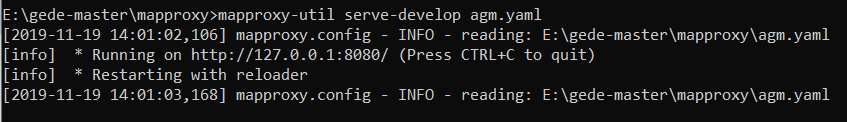
\includegraphics[width=12cm]{figures/Tugas5/1174084/1.png}
		\centering
		\caption{Start server MapProxy}
	\end{figure}
    \item Buka file contoh penggunaan LeafletJS yaitu basic.html di dalam folder leafletjs di dalam folder gede
    \hfill\break
    \begin{figure}[H]
		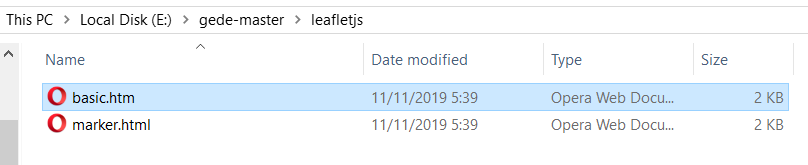
\includegraphics[width=12cm]{figures/Tugas5/1174084/2.png}
		\centering
		\caption{File Basic.html}
	\end{figure}
	\begin{figure}[H]
		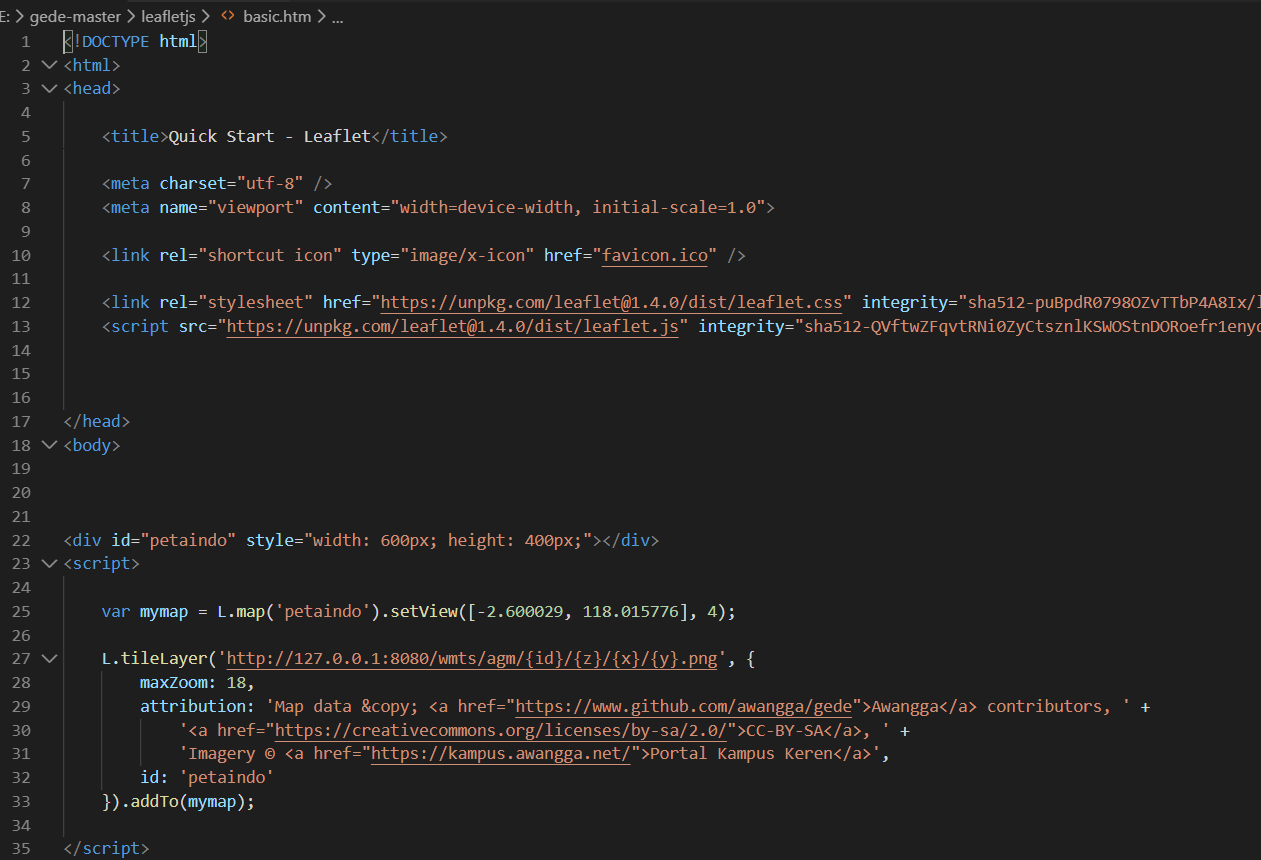
\includegraphics[width=12cm]{figures/Tugas5/1174084/7.png}
		\centering
		\caption{Code Basic.html}
	\end{figure}
    \item Lalu buka file tersebut di browser, maka hasilnya akan seperti ini
    \hfill\break
    \begin{figure}[H]
		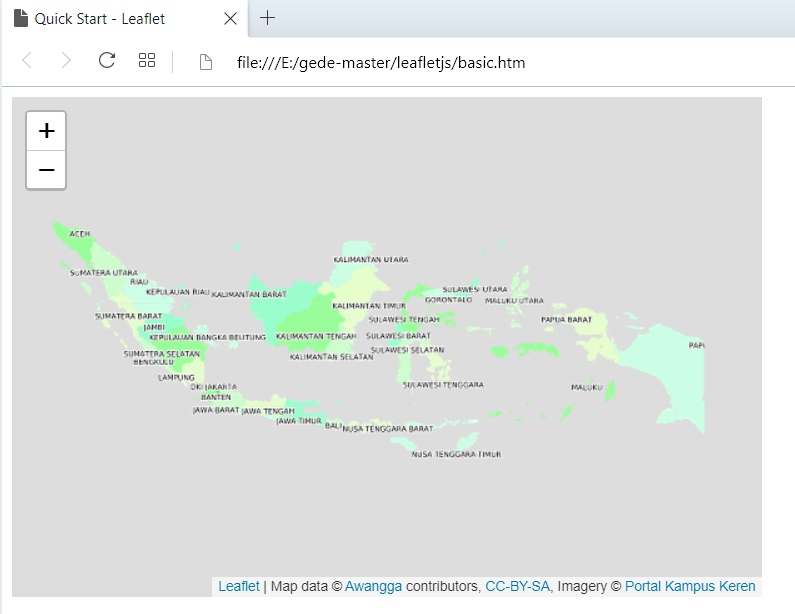
\includegraphics[width=12cm]{figures/Tugas5/1174084/3.png}
		\centering
		\caption{Tampilan Basic.html}
	\end{figure}
    \item Dengan leafletjs kita juga dapat menambahkan marker,circle, ataupun polygon dengan cara menggunakan seperti di gambar, contoh ini diambil dari file contoh kedua yaitu marker.html dari folder gede 
    \hfill\break
    \begin{figure}[H]
		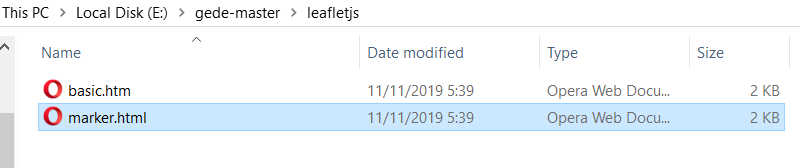
\includegraphics[width=12cm]{figures/Tugas5/1174084/4.png}
		\centering
		\caption{File Marker.html}
	\end{figure}
	\begin{figure}[H]
		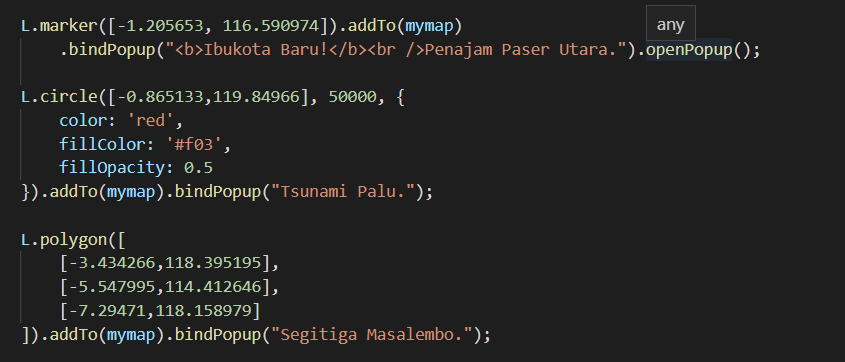
\includegraphics[width=12cm]{figures/Tugas5/1174084/6.png}
		\centering
		\caption{Code tambahan Marker.html}
	\end{figure}
    \item Lalu buka file tersebut dengan browser dan hasilnya akan seperti pada di gambar
    \hfill\break
    \begin{figure}[H]
		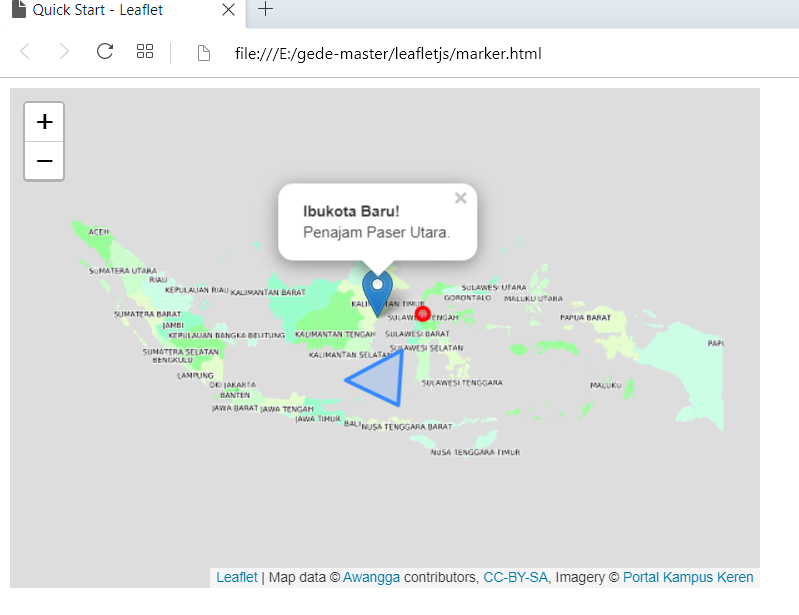
\includegraphics[width=12cm]{figures/Tugas5/1174084/5.png}
		\centering
		\caption{Tampilan Marker.html}
	\end{figure}
\end{enumerate}
\subsection{Link Youtube}
https://youtu.be/obQV7GIeNwQ